% *********************************************************************
% © 2010–2026 Jeremy Sylvestre
%
% Permission is granted to copy, distribute and/or modify this document
% under the terms of the GNU Free Documentation License, Version 1.3 or
% any later version published by the Free Software Foundation; with no
% Invariant Sections, no Front-Cover Texts, and no Back-Cover Texts. A
% copy of the license is included in the appendix entitled “GNU Free
% Documentation License” that appears in the output document of this
% PreTeXt source code. All trademarks™ are the registered® marks of
% their respective owners.
%
% *********************************************************************

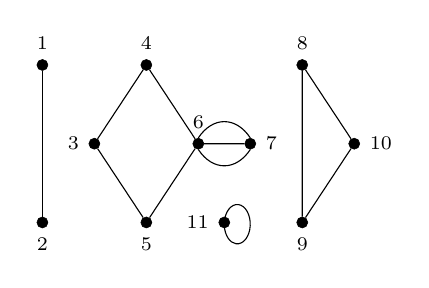
\begin{tikzpicture}[
	xscale=0.66,
	vertex/.style={ circle, draw, very thin, fill, inner sep=0pt, minimum size=4pt },
	vertexg/.style={ black!40!white, circle, draw, very thin, fill, inner sep=0pt, minimum size=4pt },
	vertexo/.style={ circle, draw, very thin, inner sep=0pt, minimum size=4pt }
]

\node at (0,2) (one) [vertex,label=above:$\scriptstyle 1$] {};
\node at (0,0) (two) [vertex,label=below:$\scriptstyle 2$] {};
\draw (one) to (two);

\node at (1,1) (three) [vertex,label=left:$\scriptstyle 3$] {};
\node at (2,2) (four) [vertex,label=above:$\scriptstyle 4$] {};
\node at (2,0) (five) [vertex,label=below:$\scriptstyle 5$] {};
\node at (3,1) (six) [vertex,label=above:$\scriptstyle 6$] {};
\node at (4,1) (seven) [vertex,label=right:$\scriptstyle 7$] {};
\draw (six) to (five) to (three) to (four) to (six) to (seven);

\draw (six.north) to [out=45,in=135] (seven.north);
\draw (six.south) to [out=315,in=225] (seven.south);

\node at (5,2) (eight) [vertex,label=above:$\scriptstyle 8$] {};
\node at (5,0) (nine) [vertex,label=below:$\scriptstyle 9$] {};
\node at (6,1) (ten) [vertex,label=right:$\scriptstyle 10$] {};
\draw (eight) to (nine) to (ten) to (eight);

\node at (3.5,0) (eleven) [vertex,label=left:$\scriptstyle 11$] {};
\draw (eleven) arc (175:-175:0.25cm) -- (eleven);


\end{tikzpicture}
